\documentclass[11pt]{beamer}
\usetheme{Warsaw}
\usepackage[utf8]{inputenc}
\usepackage{amsmath}
\usepackage{amsfonts}
\usepackage{amssymb}
\usepackage{graphicx}

\author{Aayush Goyal / Ritwik Sahani}
\title{AI and ML project}
%\setbeamercovered{transparent} 
%\setbeamertemplate{navigation symbols}{} 
\bigskip 
\bigskip 


\institute{IIT Hyderabad} 
 
%\subject{} 
\begin{document}

\begin{frame}
\titlepage
\textbf{}
\end{frame}

%\begin{frame}
%\tableofcontents
%\end{frame}
\begin{frame}
\bigskip 
\textbf{Problem - }
\linebreak 
\textsf{Q) Locus of centroid of the triangle whose vertices are (a cos t, a sin t), (b sin t, − b cos t) and (1, 0), where t is a parameter, is
\linebreak 
\textsf{}
\linebreak
(A) (3x-1)^2 + (3y)^2 = a^2 − b^2
\linebreak 
(B) (3x-1)^2 + (3y)^2 = a^2 + b^2
\linebreak 
(C) (3x + 1) + (3y) = a + b
\linebreak 
(D) (3x + 1)^2 + (3y)^2 = a^2 − b^2}
\end{frame}
\begin{frame}{•}
 \textsf{Q)} \textsf{ }\textsf{A = }$ \begin{bmatrix}
acost \\
asint 
\end{bmatrix}  $ \textsf{ }  \textsf{ } \textsf{  } \textsf{ }\textsf{B = }$ \begin{bmatrix}
asint \\
-acost 
\end{bmatrix}  $ \textsf{ }  \textsf{ }  \textsf{ }  \textsf{ } \textsf{C = }$ \begin{bmatrix}
1 \\
0 
\end{bmatrix}  $ 
\linebreak 
\bigskip 
\textsf{ }\textsf{ }\textsf{ }\linebreak\textsf{ }\textsf{where t = pi*}$ \begin{bmatrix}
0 & \frac{2}{100} & \frac{4}{100} & . & . & . & . & . & . & 2 
\end{bmatrix}  $
\\
\bigskip 
\bigskip 
\textsf{Find matrix G that is the centroid?}$
$\end{frame}
\begin{frame}
\begin{figure}
  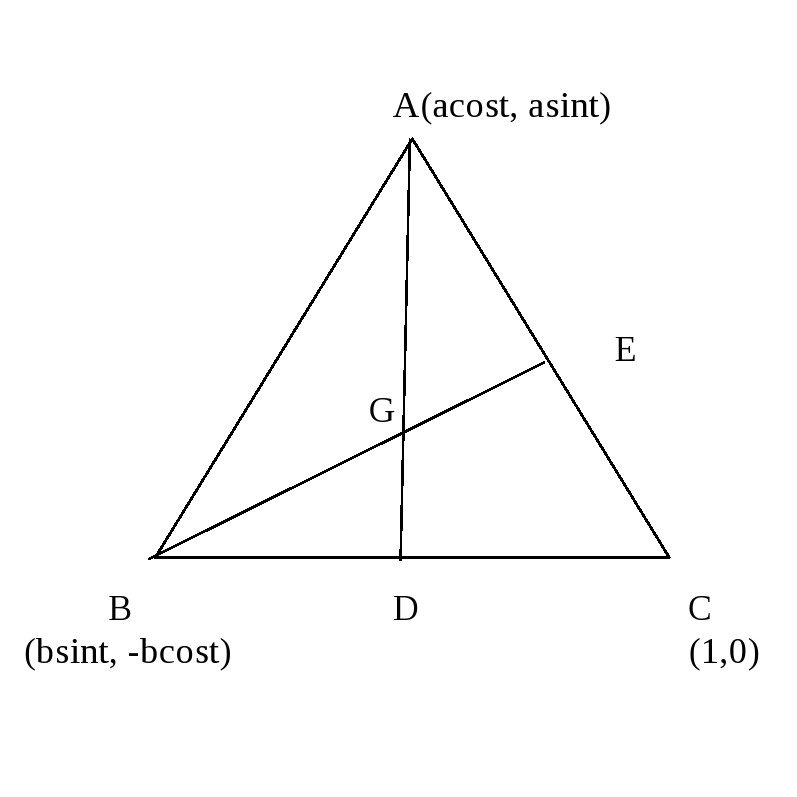
\includegraphics[width=200]{fig1.jpg}
  \caption{Figure }
  \label{fig:plot}
\end{figure}
\end{frame}
\begin{frame}
\textbf{Solution through Matrix}
\linebreak
\textsf{}
\linebreak
\textsf{} \textsf{ }\textsf{A = }$ \begin{bmatrix}
acost \\
asint 
\end{bmatrix}  $ \textsf{ }  \textsf{ } \textsf{  } \textsf{ }\textsf{B = }$ \begin{bmatrix}
asint \\
-acost 
\end{bmatrix}  $ \textsf{ }  \textsf{ }  \textsf{ }  \textsf{ } \textsf{C = }$ \begin{bmatrix}
1 \\
0 
\end{bmatrix}  $ 
\linebreak
\textsf{}
\linebreak

\textsf{D = mid point of BC = } $ \begin{bmatrix}
(asint+1)/2 \\
-acost/2 
\end{bmatrix}  $

\linebreak
\textsf{}
\linebreak

\textsf{E = mid point of AC = } $ \begin{bmatrix}
(acost+1)/2 \\
asin/2 
\end{bmatrix}  $
\linebreak
\textsf{}
\linebreak

\textsf{AD = } $ \begin{bmatrix}
(2acost - bsint -1)/2 \\
(2asint+bcost)/2 
\end{bmatrix}  $
\linebreak
\textsf{}
\linebreak

\textsf{BE = } $ \begin{bmatrix}
(2bsint - acost -1)/2 \\
(-2bcost-asint)/2 
\end{bmatrix}  $


\end{frame}
\begin{frame}
\textsf{N = (n1,n2)} $ \begin{bmatrix}
-(2asint+bcost)/2 & (2bcost+asint)/2\\
(2acost-bsint-1)/2 & (2bsint-acost-1)/2 
\end{bmatrix}  $
\linebreak
\textsf{}
\linebreak

\textsf{N^T = } $ \begin{bmatrix}
-(2asint+bcost)/2 & (2acost-bsint-1)/2\\
(2bcost+asint)/2 &  (2bsint-acost-1)/2 
\end{bmatrix}  $
\linebreak
\textsf{}
\linebreak

\textsf{P = [P1,P2]   P1 = n^T_{AD}(A)\medskip P2 = n^T_{BE}(B)\linebreak  \linebreak}  \textsf{On calculating  P1, P2 and P \linebreak }\linebreak
\textsf{}\linebreak
 \textsf{P1 = -1/2 (ab+asint)   P2 = 1/2(ab+bcost) } 
\linebreak


\textsf{P = } $ \begin{bmatrix}
-a/2(b+sint) \\
b/2(a+cost)  
\end{bmatrix}  $

\end{frame}
\begin{frame}
\textsf{\textbf{Final Answer} \linebreak$ Centroid = G = (N^T)^{-1}(P) =  $}$  \begin{bmatrix}
(acost+bsint+1)/3 \\
(asint-bcost)/3 
\end{bmatrix}  $

\end{frame}
\begin{frame}
\begin{figure}
  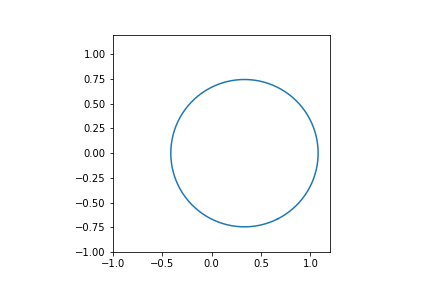
\includegraphics[width=\linewidth]{plot.png}
  \caption{Locus Plot \textit{$(3x-1)^2 + (3y)^2 = 5}$}
  \label{fig:plot}
\end{figure}

\end{frame}



\end{document}